\documentclass{beamer}

\mode<presentation> {
	\usetheme{Berlin}
}

\title[Numerical Methods for Scientific Computations and Advanced Applications, Hissarya, Bulgaria]{
	Artificial Neural Network Activation Function Optimization with Genetic Algorithms
}

\author{Ivan Blagoev, Janeta Sevova, Kolyu Kolev}

\date{28-31.V.2018}

\institute[IICT-BAS, NMSCAA'18] {
	Institute of Information and Communication Technologies \\ 
	Bulgarian Academy of Sciences \\
	\medskip
	\textit{i.blagoev@iit.bas.bg}
}

\begin{document}

\begin{frame}
\titlepage
\end{frame}

\begin{frame}
\frametitle{Overview}
\tableofcontents
\end{frame}

\section{Introduction}

\subsection{Artificial Neural Networks}

\begin{frame}
\frametitle{What ANNs are?}
\begin{itemize}
  \item Common tool in machine learning.
  \item Brain-inspired systems which are intended to replicate the way that we humans learn.
  \item Consist of input and output layers and a hidden layer(s) consisting of units that transform the input into something that the output layer can use.
\end{itemize}
\end{frame}

\begin{frame}
\frametitle{ANN Example}
\begin{figure}[h]
  \centering
  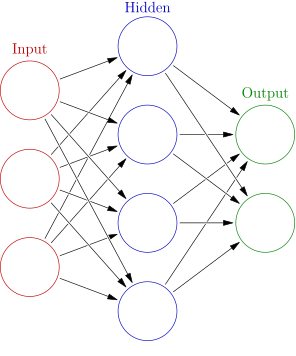
\includegraphics[width=0.5\linewidth]{fig02}
\label{fig:02}
\end{figure}
\end{frame}

\subsection{Signals Transmission}

\begin{frame}
\frametitle{Transmission}
\begin{itemize}
  \item The most used transmission function is the linear function:
  \begin{equation}
  \label{equation01}
  y_{j} = \sum_{i=1}^{} x_{i}*w_{ij}
  \end{equation}
  \begin{itemize}
    \item First problem is that the number of multiplications can be high, but worse is that it can vary.
    \item The second problem is that values of the weight can go to big positive numbers or big negative numbers.
  \end{itemize}
  \item In order signals to be usable additional computation is needed in form of normalization. 
\end{itemize}
\end{frame}

\begin{frame}
\frametitle{Activation}
\begin{itemize}
  \item The most used activation functions are the sigmoid and hyperbolic tangent functions:

  \begin{equation}
  \label{equation02}
  z_{j} = \frac{1}{1 + e^{-y_{j}}}
  \end{equation}
  \begin{itemize}
    \item The output range is from 0.0 to 1.0.
  \end{itemize}
  
  \begin{equation}
  \label{equation03}
  z_{j} = \frac{e^{2y_{j}}-1}{e^{2y_{j}}+1}
  \end{equation}
  \begin{itemize}
    \item The output range is from -1.0 to +1.0.
  \end{itemize}
\end{itemize}
\end{frame}

\subsection{Neuron Activation Function}

\begin{frame}
\frametitle{List of Popular Activation Functions}
\begin{figure}[h]
  \centering
  \includegraphics[width=0.5\linewidth]{fig01}
\label{fig:01}
\end{figure}
\end{frame}

\section{Technical Proposition}

\subsection{Genetic Programming}

\begin{frame}
\frametitle{Activation Function Optimization}
\begin{itemize}
  \item Similar idea is used in artificial neural networks with radial basis functions.
  \item Genetic algorithms are involved in neurons activation function optimization.
  \item The goal is to find activation function mathematical expression. 
  \begin{itemize}
    \item To reduce ANN training time. 
    \item No lost of ANN operation accuracy.
  \end{itemize}
\end{itemize}
\end{frame}

\begin{frame}
\frametitle{Programming Frameworks Used}
\begin{itemize}
  \item Encog Machine Learning Framework
  \begin{itemize}
    \item Multilayer perceptron representation.
    \item Alternative activation function capabilities.
  \end{itemize}
  \item mXparser Math Expression Library
  \begin{itemize}
    \item Mathematical expressions representation.
    \item Mathematical expressions evaluation.
  \end{itemize}
  \item Apache Genetic Algorithms Framework
  \begin{itemize}
    \item Problem related chromosomes representation.
    \item Evolutionary operations (crossover, mutation and selection).
  \end{itemize}
\end{itemize}
\end{frame}

\section{Conclusions}

\subsection{Advantages and Disadvantages}

\begin{frame}
\frametitle{Conclusions}
\begin{itemize}
  \item Findings for alternative activation functions can lead to speed-up of ANN training.
\end{itemize}
\end{frame}

\subsection{Q\&A}

\begin{frame}
\frametitle{Questions and Answers}
\center \huge{Thank you for the attention!}
\end{frame}

\end{document}
